\begin{outline-text-1}
15 min + 5 min question

POSTER 4ft (122cm) wide x 6ft (183 cm) tall

\begin{larger}
\begin{center}
Masataro Asai

2nd year in Ph.D program (2 years to go)

University of Tokyo

 

Short talk (15min)
\end{center}
\end{larger}
\end{outline-text-1}

\section{Overview}
\label{sec-1}

\begin{itemize}
\item What I've been doing (5 min)
\begin{itemize}
\item primarily in classical planning
\item Briefly summarize 3 papers
\end{itemize}
\item How to form a clean thesis \& what I'm insterested in (10 min)
\begin{itemize}
\item To construct a consistent story →
\item \emph{Theory unifying all satisficing heuristic search}
\item \emph{4th paper} : aiming to be a non ad-hoc macro paper
\end{itemize}
\end{itemize}

\section{}
\label{sec-2}

\begin{xlarge}
\begin{center}
Prior Work
\end{center}
\end{xlarge}

\section{CELL-ASSEMBLY system}
\label{sec-3}

\begin{note}
Asai, M.; Fukunaga, A: 2014. Fully Automated Cyclic Planning for Large-Scale Manufacturing Domains. In ICAPS2014.
\end{note}

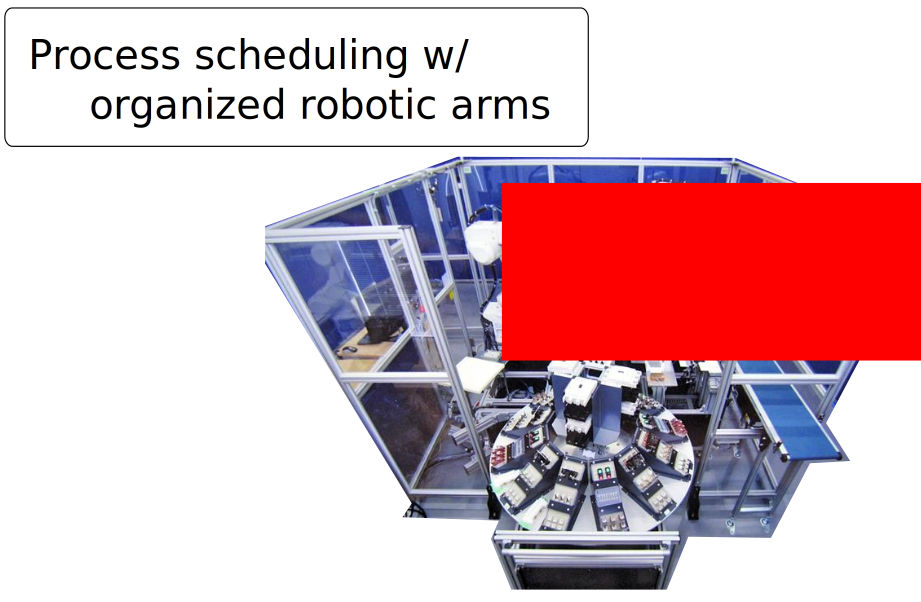
\includegraphics{img/assemble-icaps14-intro.png}

\subsection{Issues addressed}
\label{sec-3-1}

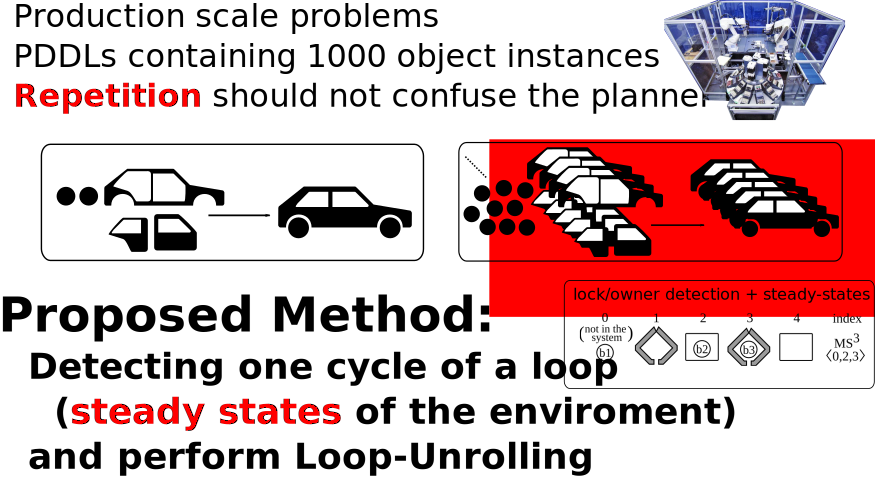
\includegraphics{img/assemble-icaps14.png}

\section{ICAPS15 paper}
\label{sec-4}

\begin{resume}
In this work, we generalized the proposed method by detecting and
categorizing the logical structure which forms each loop.
For example, programs do not know that cars consists of several parts such as doors, engines and tires.
\end{resume}

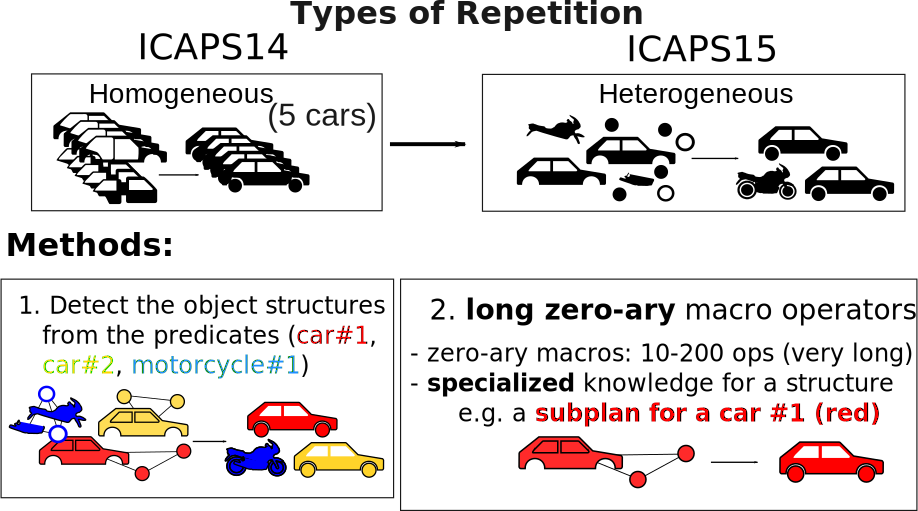
\includegraphics{img/assemble-keps14-icaps15.png}

\begin{note}
Asai, M.; Fukunaga, A: 2015. Solving Large-Scale Planning Problems by Decomposition and Macro Generation. In ICAPS2015.
\end{note}

\section{AAAI16 paper (visit my 2nd poster session)}
\label{sec-5}

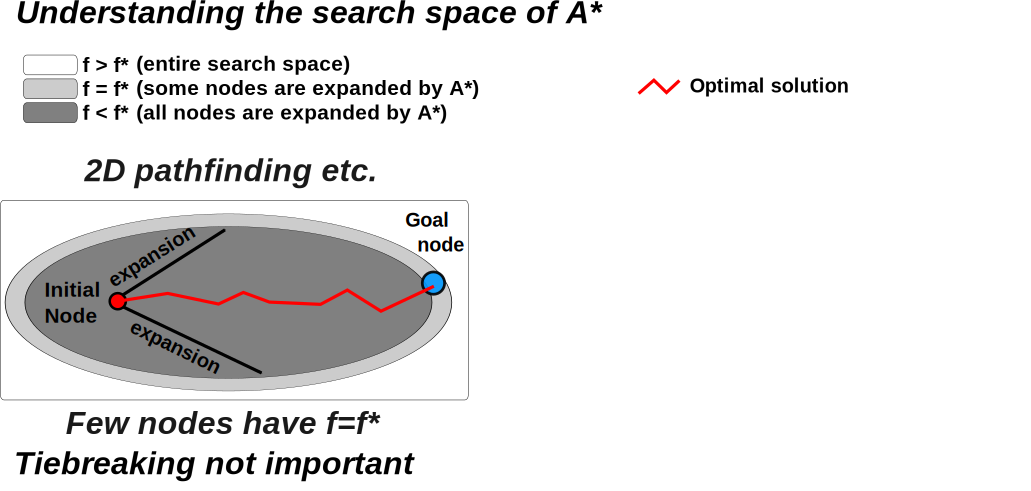
\includegraphics{img/aaai16-1-1.png}

\begin{note}
Asai, M.; Fukunaga, A: 2016. Tiebreaking Strategies for A* Search: How to Explore the Final Frontier. In AAAI-2016.
\end{note}

\subsection{AAAI16 paper (visit my 2nd poster session)}
\label{sec-5-1}


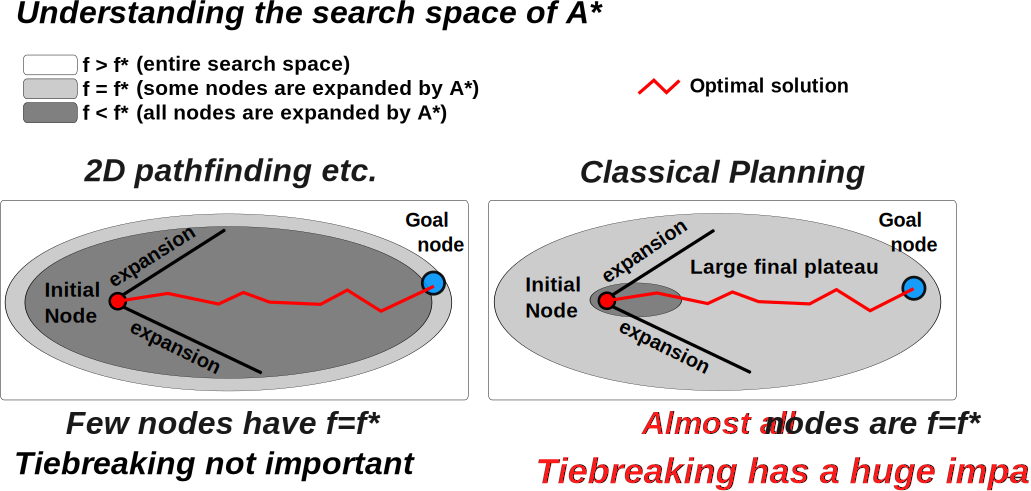
\includegraphics{img/aaai16-1-2.png}

\begin{note}
Asai, M.; Fukunaga, A: 2016. Tiebreaking Strategies for A* Search: How to Explore the Final Frontier. In AAAI-2016.
\end{note}

\subsection{Investigating \emph{h}-tiebreaking in A*}
\label{sec-5-2}

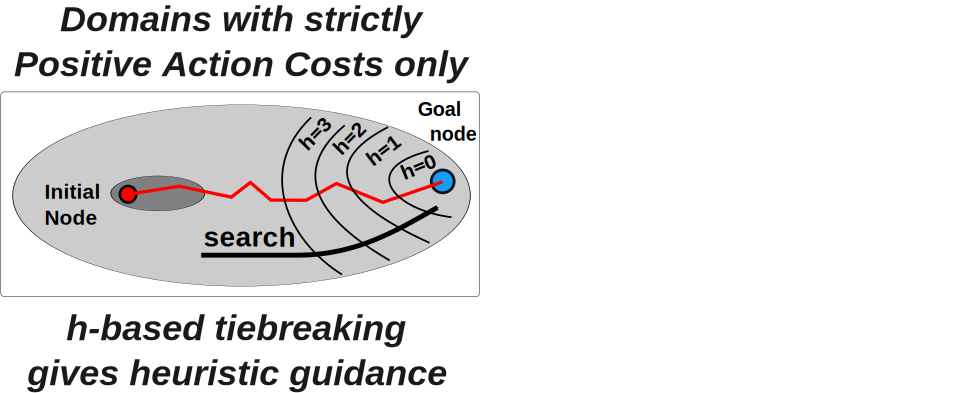
\includegraphics{img/aaai16-2.png}

\subsection{Investigating \emph{h}-tiebreaking in A*}
\label{sec-5-3}

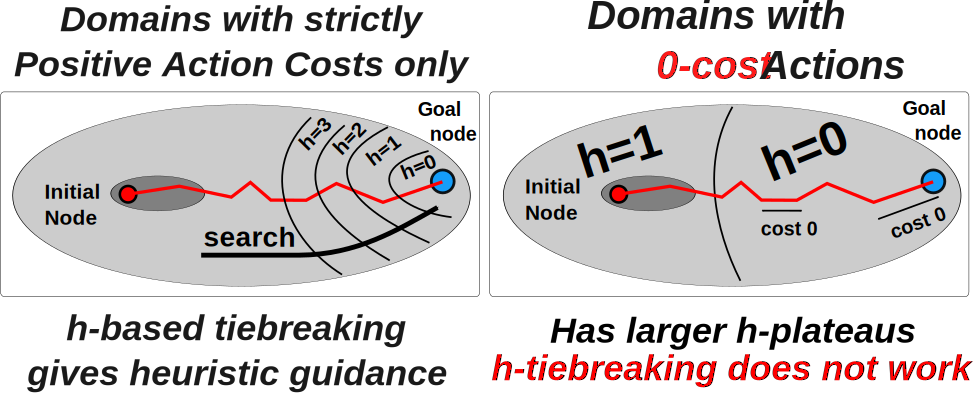
\includegraphics{img/aaai16-2-1.png}

\subsection{Investigating \emph{h}-tiebreaking in A*}
\label{sec-5-4}

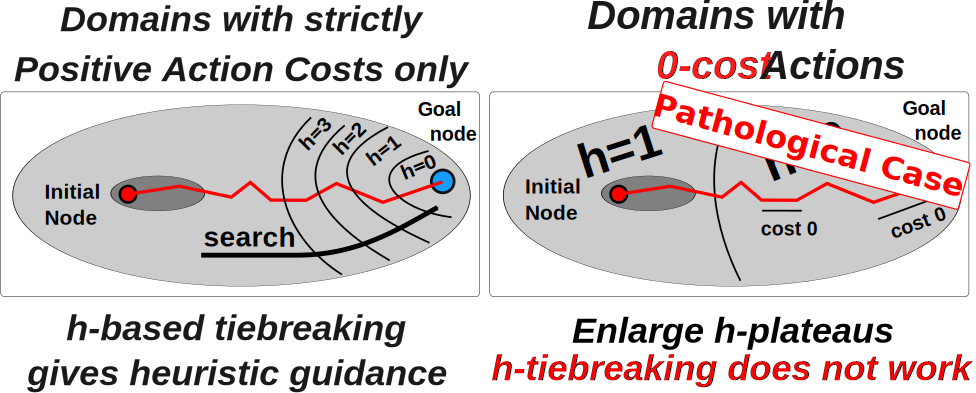
\includegraphics{img/aaai16-2-2.png}

\subsection{Investigating \emph{h} + LIFO/FIFO tiebreaking in A*}
\label{sec-5-5}

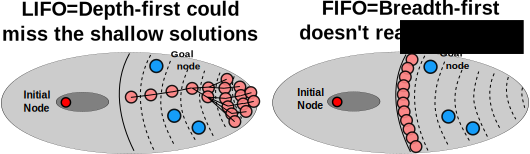
\includegraphics{img/plateau-3-0.png}

\subsection{Investigating \emph{h} + LIFO/FIFO tiebreaking in A*}
\label{sec-5-6}

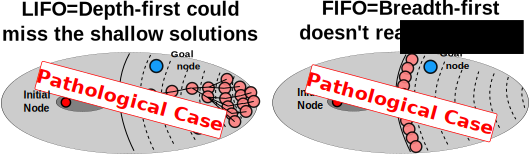
\includegraphics{img/plateau-3-1.png}

\subsection{A* with \emph{h} + Depth Diversification}
\label{sec-5-7}

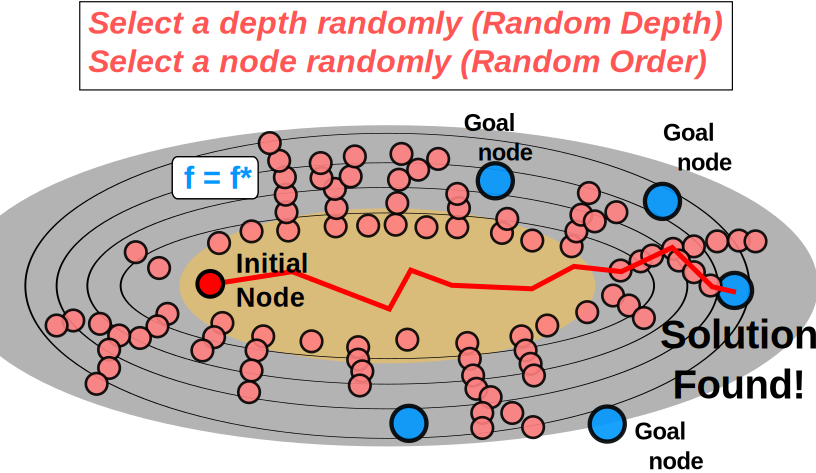
\includegraphics{img/aaai16-3.png}

annd "plateau search = satisficing planning"

\section{}
\label{sec-6}

\begin{xlarge}
\begin{center}
Future Work

 
\end{center}
\end{xlarge}

 

 

\section{Earmuffs Required}
\label{sec-7}

\begin{xlarge}


\begin{center}
Future Work

== Research IDEAs : not yet fully developped
\end{center}
\begin{alignright}

\end{alignright}
\end{xlarge}

\section{Toward Thesis Proposals}
\label{sec-8}

\begin{larger}
1st, 2nd paper: \textbf{Macros}, satisficing search

3rd paper: A*, tiebreaking, \textbf{plateau}, optimising search

\begin{alignright}
→ Weak connections between the topics

Requires a unified story
\end{alignright}

\begin{center}
\begin{itemize}
\item \textbf{(macro ∩ plateau analysis) == search space}
\end{itemize}
\end{center}
\end{larger}


\section{A* tiebreaking [RD RO] paper was about search space}
\label{sec-9}

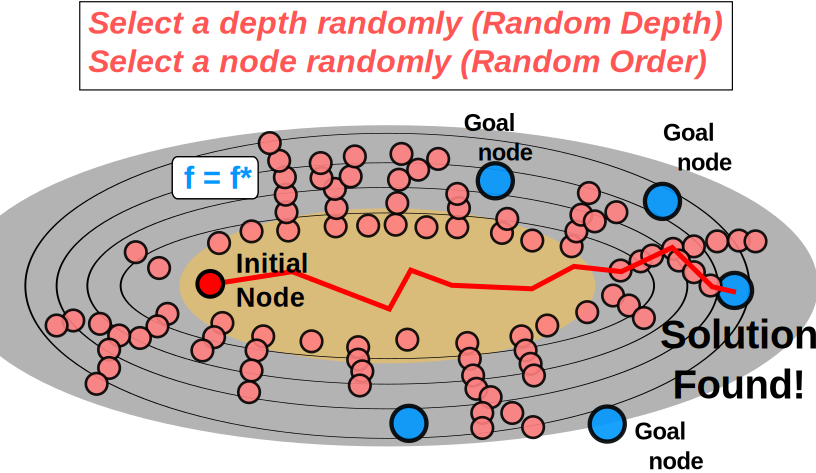
\includegraphics{img/aaai16-3.png}

\section{Macro operators changes the search space structure}
\label{sec-10}

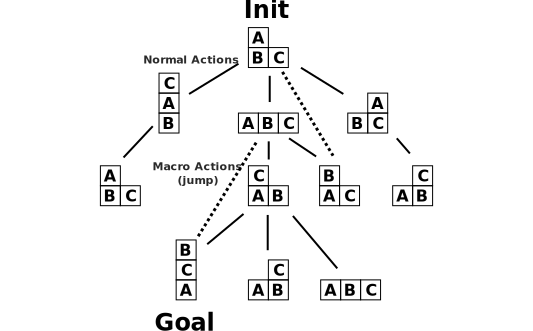
\includegraphics{img/macro/search0.png}

\section{Macro operators changes the search space structure}
\label{sec-11}

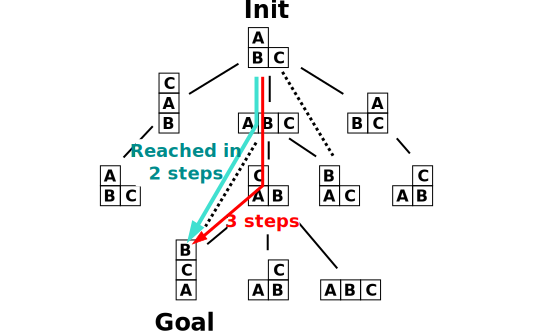
\includegraphics{img/macro/search1.png}

\section{Proposal: Unifying Framework for Analyzing Search Space}
\label{sec-12}

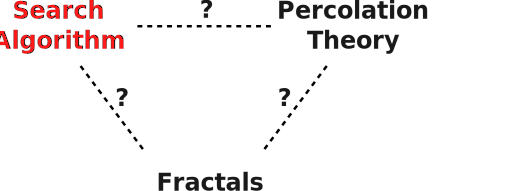
\includegraphics{img/triangle.png}

\section{Proposal: Unifying Framework for Analyzing Search Space}
\label{sec-13}

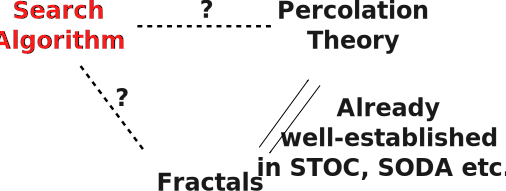
\includegraphics{img/triangle0.png}

\section{Proposal: Unifying Framework for Analyzing Search Space}
\label{sec-14}

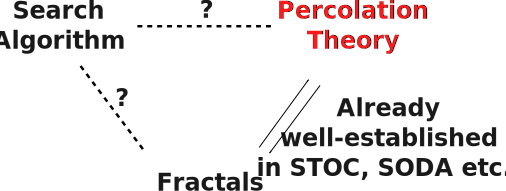
\includegraphics{img/triangle1.png}

\section{}
\label{sec-15}

\begin{xlarge}
\begin{center}
Percolation Theory
\end{center}
\end{xlarge}

\subsection{Example: Percolation in 2-dimentional grids}
\label{sec-15-1}

A node is either \textbf{occupied} or \textbf{unoccupied}

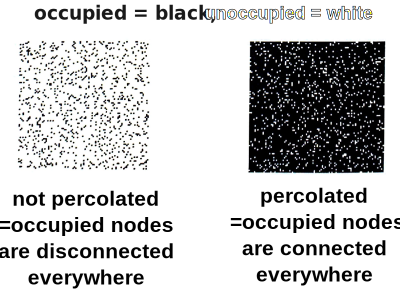
\includegraphics{img/percolate/percolated0.png}

\begin{alignright}
\begin{larger}
\begin{itemize}
\item Key interst: \textbf{when/how} a graph percolates?
\end{itemize}
\end{larger}
\end{alignright}

\subsection{Bond (edge) / Site (node) percolation}
\label{sec-15-2}

\url{img/static/site-bond.gif}

\subsection{Percolation described by occupation ratio \emph{r}}
\label{sec-15-3}

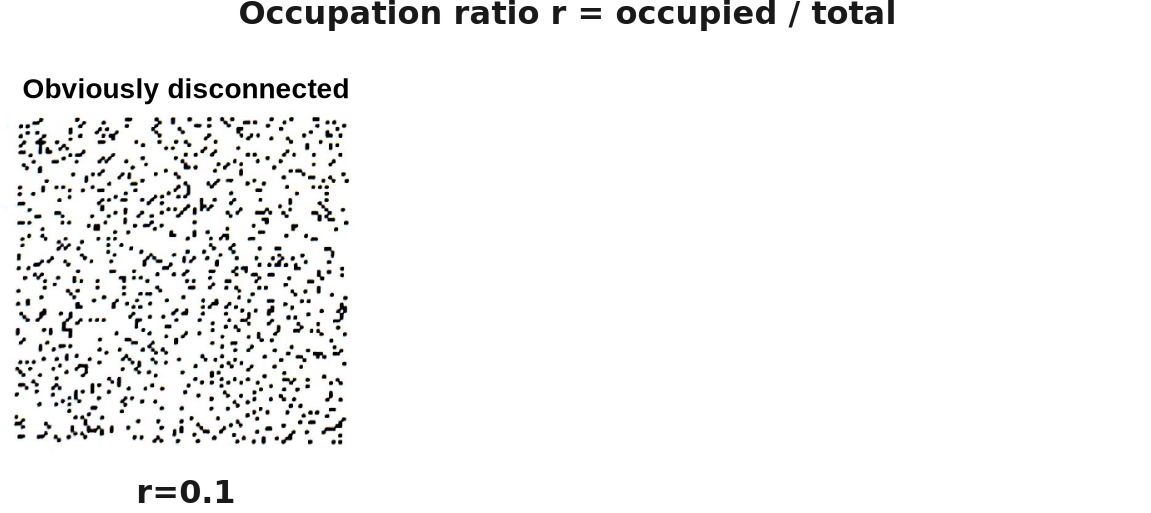
\includegraphics{img/percolate/cluster0.png}

\subsection{Percolation described by occupation ratio \emph{r}}
\label{sec-15-4}

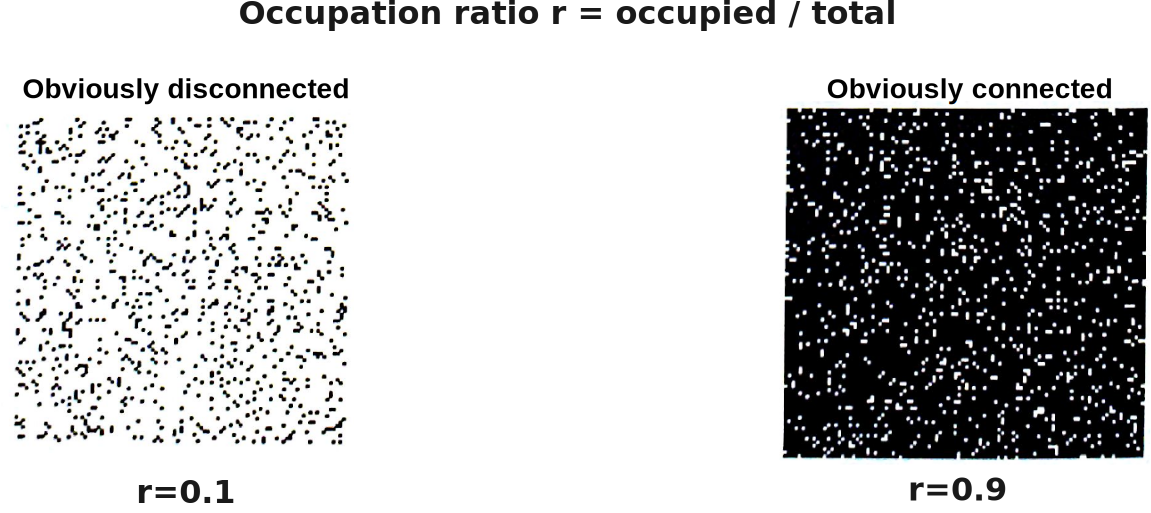
\includegraphics{img/percolate/cluster1.png}

\subsection{Percolation described by occupation ratio \emph{r}}
\label{sec-15-5}

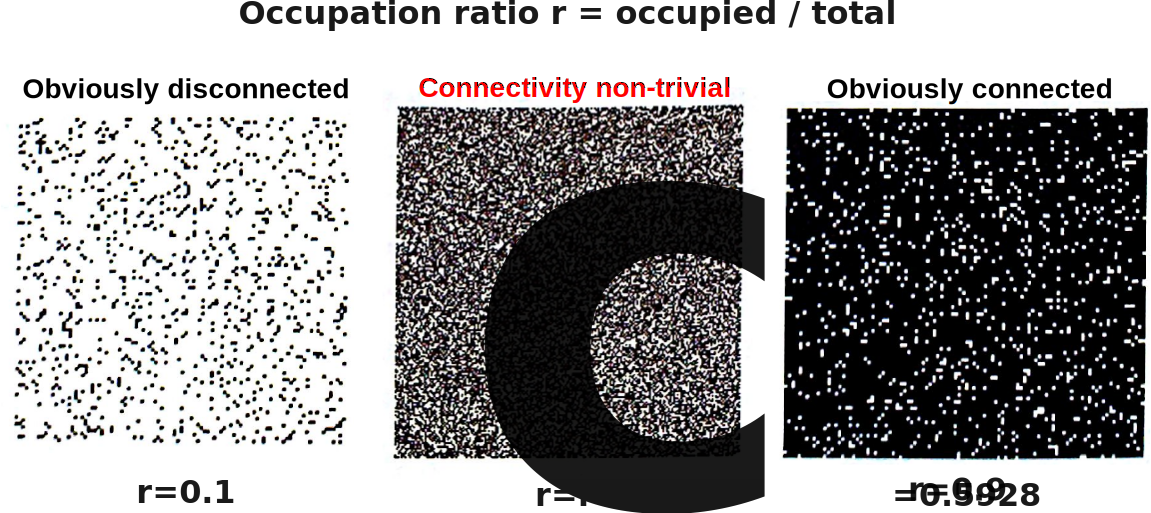
\includegraphics{img/percolate/cluster2.png}

\subsection{Percolation described by occupation ratio \emph{r}}
\label{sec-15-6}

Generates a connected cluster with complex shape

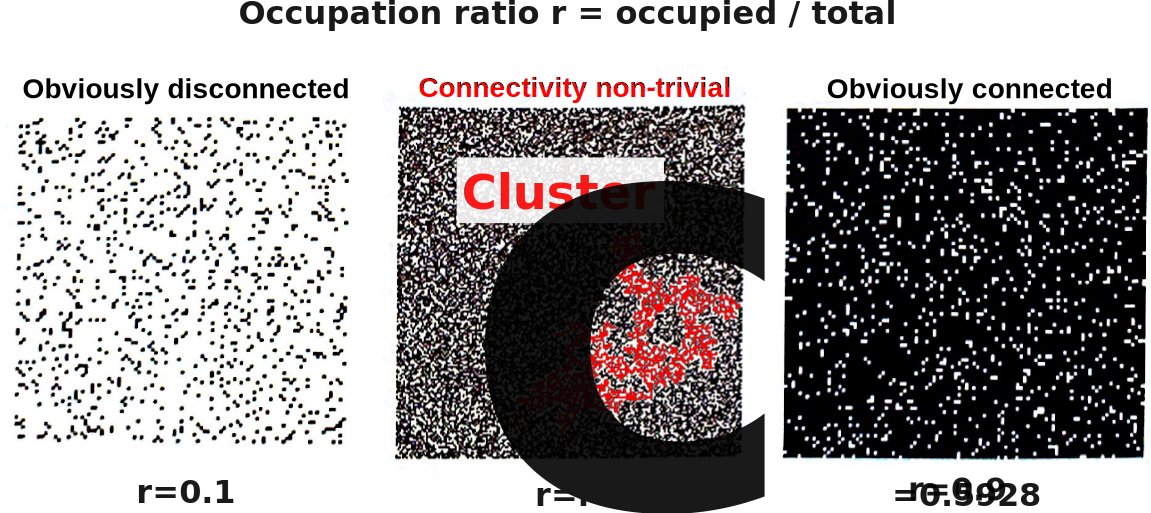
\includegraphics{img/percolate/cluster3.png}

\subsection{Phase Transition}
\label{sec-15-7}

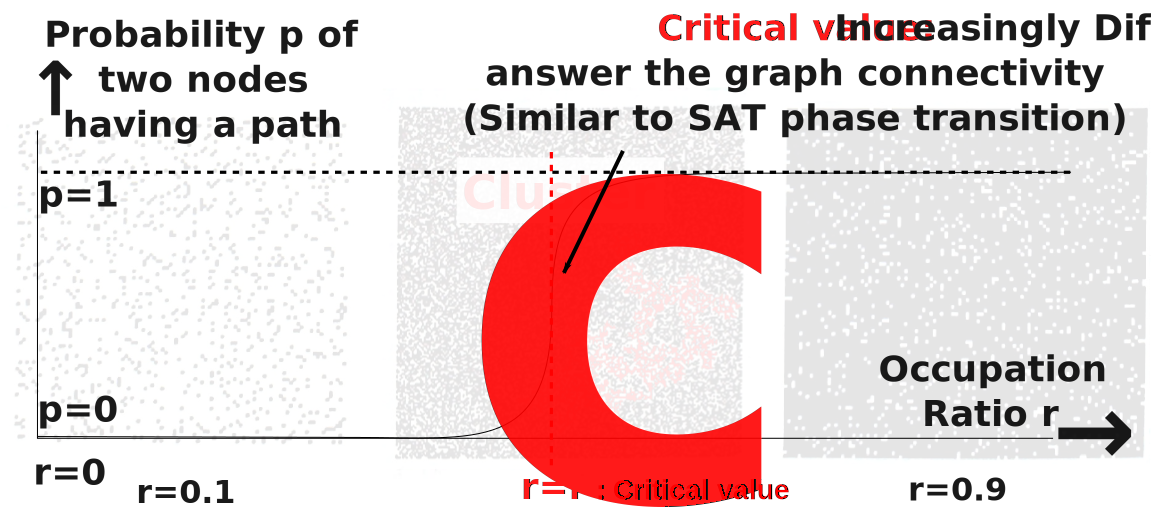
\includegraphics{img/percolate/cluster4.png}

\subsection{Macros may be shifting the ratio to the right}
\label{sec-15-8}

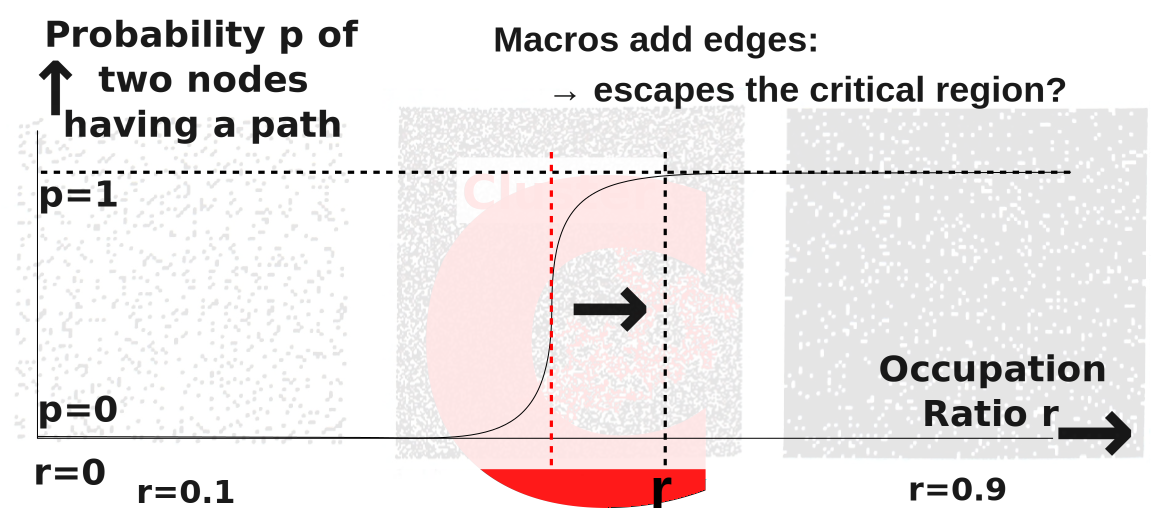
\includegraphics{img/percolate/cluster5.png}

\subsection{Forward Search : Increasing \emph{r} as the search progresses}
\label{sec-15-9}

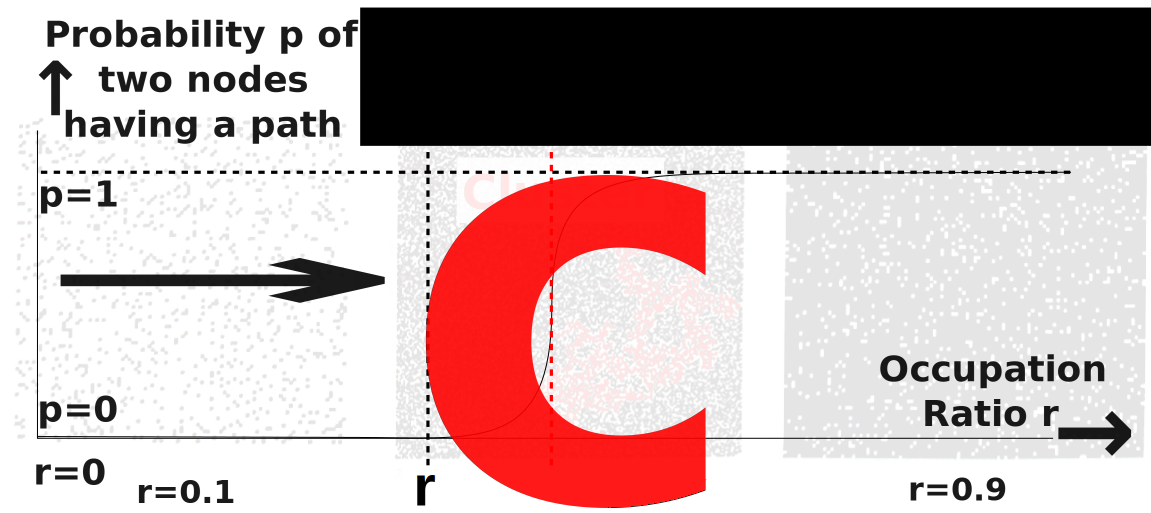
\includegraphics{img/percolate/cluster6.png}

\subsection{Open Questions}
\label{sec-15-10}

\begin{itemize}
\item \textbf{Prove the connection between macro-operators and critical value}
\begin{itemize}
\item I am testing if randomly generated \textbf{Junk Macros} improve the performance
\begin{itemize}
\item \textbf{Ongoing work --- \emph{positive results} (next slide)}
\end{itemize}
\end{itemize}
\item \textbf{How \emph{existing macro-approaches} change the connectivity?}
\begin{itemize}
\item MacroFF(Botea05), Marvin(Coles04,07) MUM(Chrpa14), CAP(Asai15), BLOMA(Siddiqui15)
\end{itemize}
\item \textbf{What is the \emph{r$_{\text{c}}$} of each domain?}
\begin{itemize}
\item critical value of Logistics is X, Barman is Y \ldots{}
\end{itemize}
\item \textbf{At which \emph{r} does each search algorithm find a solution?}
\begin{itemize}
\item Lookahead search, GBFS, Type-GBFS, A*, Random Walk\ldots{}
\end{itemize}
\end{itemize}

\subsubsection{Preliminary results on Junk Macros}
\label{sec-15-10-1}

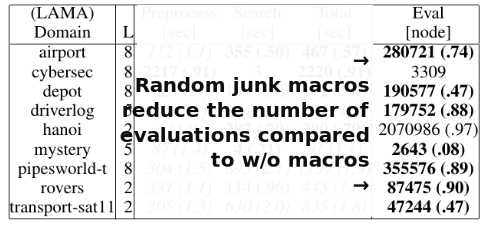
\includegraphics{img/percolate/junk.png}

\begin{alignright}
Promising direction!
\end{alignright}

\section{Unifying Framework for Analyzing Search Space}
\label{sec-16}

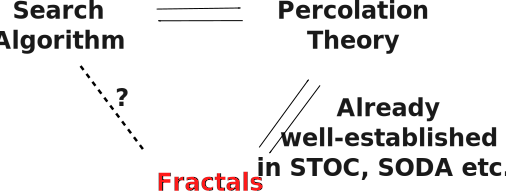
\includegraphics{img/triangle2.png}

\section{}
\label{sec-17}

\begin{xlarge}
\begin{center}
Fractals
\end{center}
\end{xlarge}

\begin{alignright}
No time, only described briefly
\end{alignright}

\subsection{Fractals}
\label{sec-17-1}

Sierpinsky's Gasket, Tree (L-system), Koch Curve


\begin{container-fluid}
\begin{row-fluid}
\begin{span6}
\url{img/static/sierpinski.gif}
\end{span6}
\begin{span6}
\url{img/static/koch.gif}
\end{span6}
\end{row-fluid}
\end{container-fluid}


\subsection{Fractal Dimension: How many nodes are included when the \textbf{\emph{scale}} changes?}
\label{sec-17-2}

Takes Fractional value; != Space Dimension

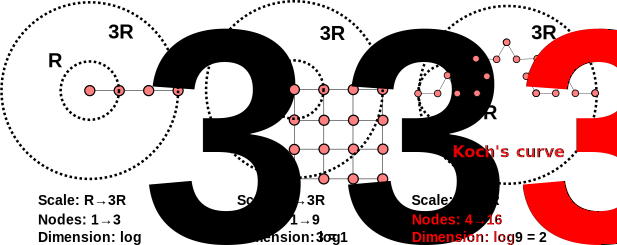
\includegraphics{img/fractals/dimention.png}

\subsection{Fractals are defined by generative rules: example}
\label{sec-17-3}

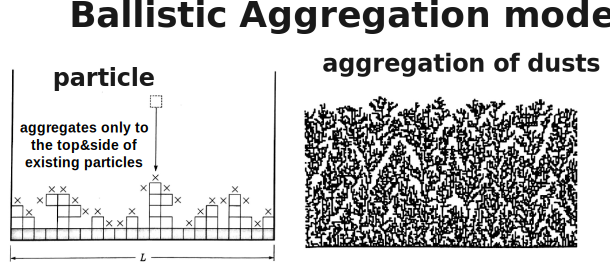
\includegraphics{img/fractals/ba.png}

\subsection{Fractals are defined by generative rules: example}
\label{sec-17-4}

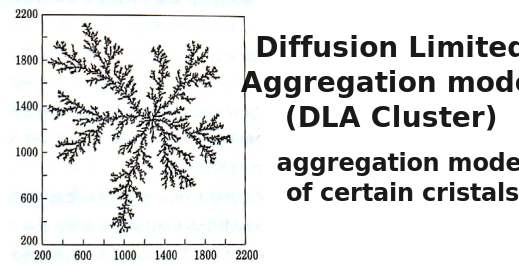
\includegraphics{img/fractals/dla.png}

\subsection{Fractals are defined by generative rules: example}
\label{sec-17-5}

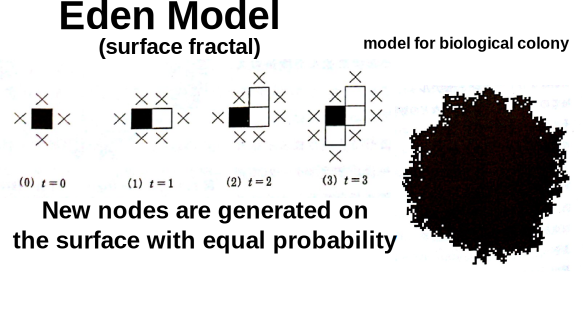
\includegraphics{img/fractals/eden.png}

\subsection{\textbf{\emph{Search space}} is also defined by expansion rules}
\label{sec-17-6}

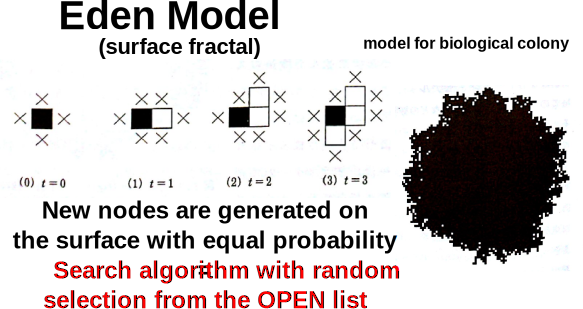
\includegraphics{img/fractals/eden-2.png}

\subsection{Connections between Fractals and Search Algorithms}
\label{sec-17-7}

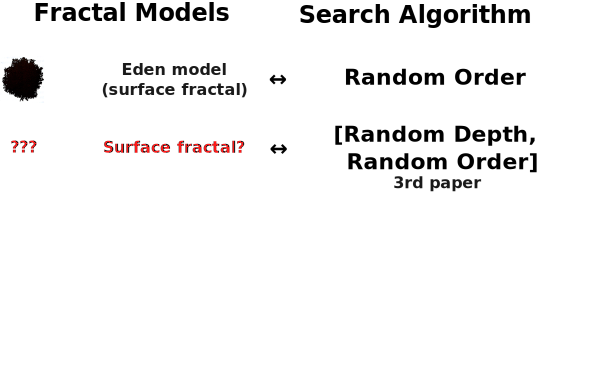
\includegraphics{img/fractals/fractal.png}

\subsection{Connections between Fractals and Search Algorithms}
\label{sec-17-8}

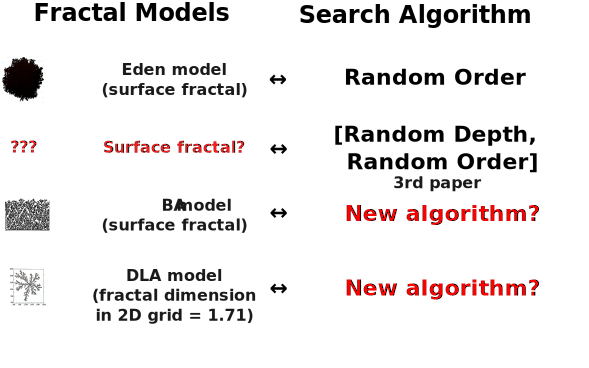
\includegraphics{img/fractals/fractal2.png}

\subsection{Connections between Fractals and Search Algorithms}
\label{sec-17-9}

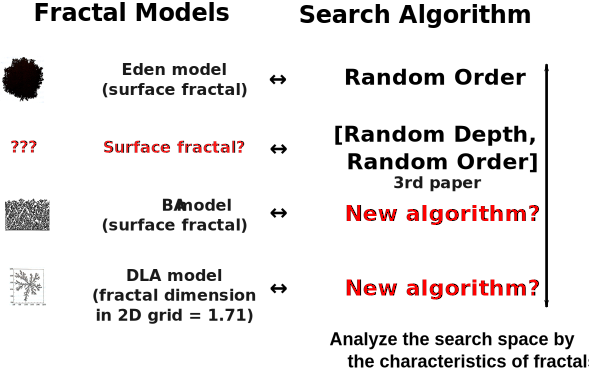
\includegraphics{img/fractals/fractal3.png}

\subsection{Connections between Fractals and Percolation}
\label{sec-17-10}

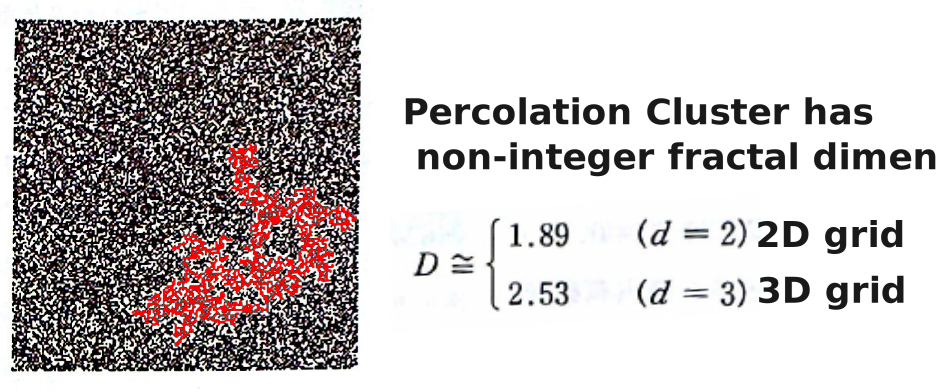
\includegraphics{img/fractals/cluster.png}

\section{Unifying Framework for Analyzing Search Space}
\label{sec-18}

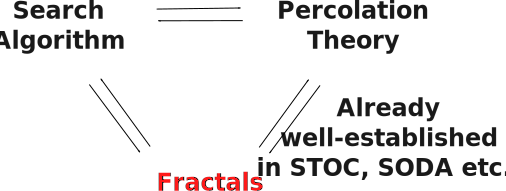
\includegraphics{img/triangle3.png}

\section{Conclusion: Thesis Abstract}
\label{sec-19}

\begin{larger}
\begin{itemize}
\item \textbf{Establish a framework} for analysing the search behavior based on percolation theory
\item \textbf{Propose paper 1,2,3}
\item \textbf{Analyze paper 1,2,3} using \textbf{percolation theory}
\begin{itemize}
\item Macro operators in paper 1,2
\item Tiebreaking mechanism in paper 3
\end{itemize}
\item \textbf{\emph{Give an answer} to why paper 1,2,3 perform good}
\end{itemize}
\end{larger}

\begin{alignright}
→ Unified, consistent thesis!
\end{alignright}

\begin{larger}
\begin{center}
Thank you for listening!
\end{center}
\end{larger}
